\documentclass[landscape]{article}
\usepackage[utf8]{inputenc}
\usepackage[T1]{fontenc}
\usepackage{microtype}

\usepackage{newspaper}
\usepackage{sudoku}
\usepackage{booktabs}
\usepackage{enumitem}
\setlist{noitemsep}
\setlist[enumerate]{label=$\circ$, leftmargin=0cm}
\setlength\heavyrulewidth{0ex} % sports scores table

\date{\today}
\currentvolume{1}
\currentissue{1}

\SetPaperName{The Daily Hennig}
\SetHeaderName{The Daily Hennig}
\SetPaperLocation{Somerville, MA}
\SetPaperSlogan{``All the News I Feel Like Printing.''}
\SetPaperPrice{Zero Dollars}

\usepackage{graphicx}
\usepackage{multicol}
\usepackage{picinpar}
\usepackage{newspaper-mod} % modifies newspaper style
\usepackage{ifthen}

\setlength\textwidth{9.5in}		% article default = 418pt
\setlength\textheight{7.0in}		% article default = 296pt

\renewcommand\headline[1]{\begin{center} {\huge \textsl{ #1}}\\ %
			\rule[5pt]{0.8\hsize}{0.5pt}\\ \end{center}}

%%%%%%%%%  Front matter   %%%%%%%%%%
\begin{document}
\maketitle

\begin{multicols}{3}
\headline{Weather}
\vspace{-0.5cm}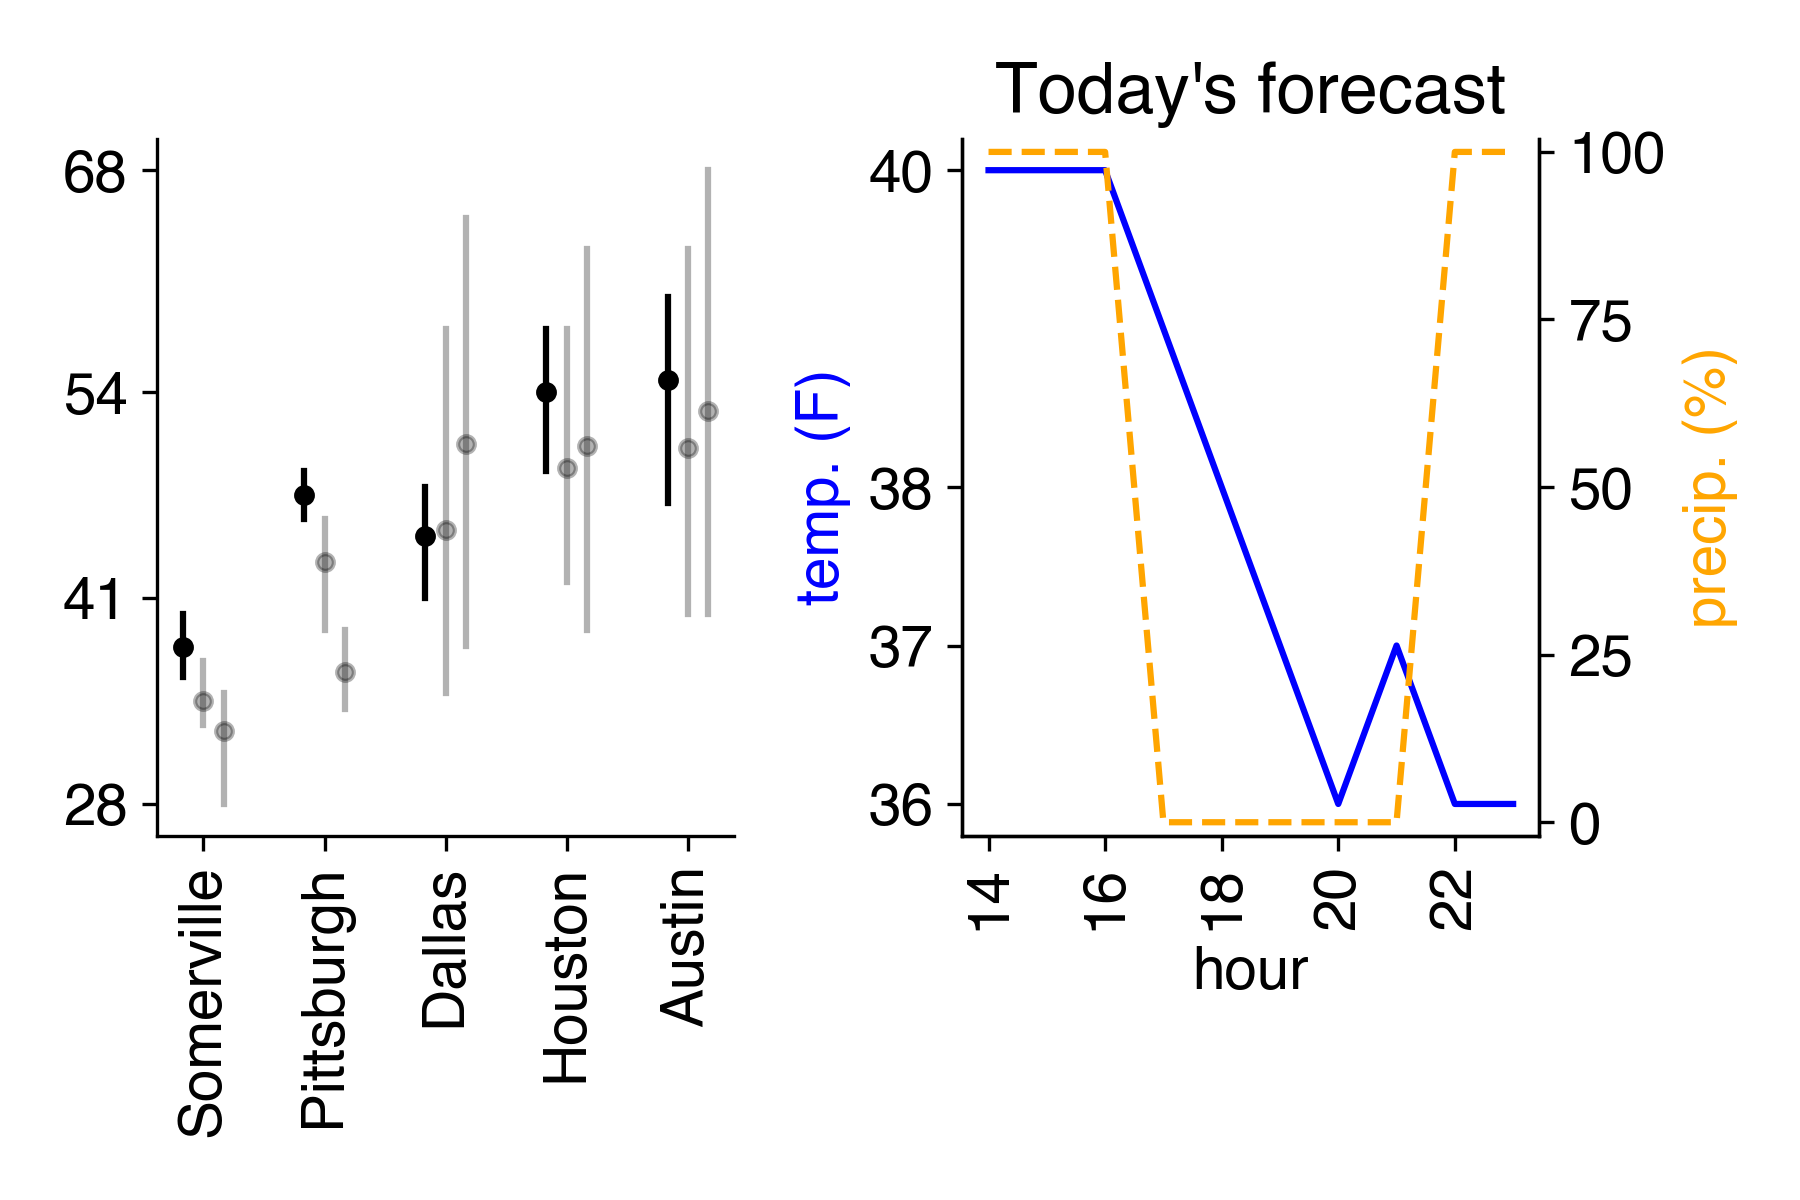
\includegraphics[width=\linewidth]{images/weather.png}

% \columnbreak
\headline{Arts \& Culture}
\vspace{-0.3cm}
\textbf{Jacqueline Novak: Get on Your Knees} (2024, Comedy/Stand-up, 1h 34m): Comedian Jacqueline Novak delivers a funny and philosophical meditation on sex, coming-of-age and a certain body part in this intimate stand-up special.. Directed by Natasha Lyonne.. Starring Jacqueline Novak, Natasha Lyonne.

\noindent\textbf{Pitchfork's Best New Album}: \textit{Almighty So 2} by Chief Keef [Rap]: The long-teased sequel to his cult-classic mixtape is a highlight in the Chicago rapper{\textquoteright}s career, bringing the first-wave drill he helped popularize screaming into the future.

\headline{Sports}
\vspace{-0.3cm}
\begin{enumerate}
\item Jokic scores 40, Nuggets shut down Edwards in 112-97 win over Wolves for a 3-2 series lead
\item Brunson scores 44, Knicks beat Pacers 121-91 to move a win away from conference finals
\item Caitlin Clark struggles early in WNBA debut before scoring 20 points in Fever{\textquoteright}s loss to Connecticut\end{enumerate}
\begin{center}
	\textbf{NBA games last night:}
\begin{tabular}{llll}
\toprule
Detroit Pistons & 120 & Oklahoma City Thunder & 104 \\
 Indiana Pacers & 116 &     Memphis Grizzlies & 110 \\
  Atlanta Hawks & 126 &       Toronto Raptors & 125 \\
\bottomrule
\end{tabular}

\end{center}
\begin{minipage}{0.1\linewidth}
	
\includegraphics[width=\linewidth]{images/mavs-logo.png}
\end{minipage}
\begin{minipage}{0.9\linewidth}
	\textbf{Dallas Mavericks}

Record: 25-20, 8th in NBA Western Conference

Next Game: Saturday, Jan. 27 vs. SAC
\end{minipage}
\begin{center}
	\textbf{NBA Standings}

\textit{Western Conference}
\begin{tabular}{llllll}
 & Team & W & L & \% & GB \\
1 & Oklahoma City Thunder & 57 & 25 & .695 & — \\
2 & Denver Nuggets & 57 & 25 & .695 & — \\
3 & Minnesota Timberwolves & 56 & 26 & .683 & 1.0 \\
4 & Los Angeles Clippers & 51 & 31 & .622 & 6.0 \\
5 & Dallas Mavericks & 50 & 32 & .610 & 7.0 \\
6 & New Orleans Pelicans & 49 & 33 & .598 & 8.0 \\
7 & Phoenix Suns & 49 & 33 & .598 & 8.0 \\
8 & Los Angeles Lakers & 47 & 35 & .573 & 10.0 \\
9 & Sacramento Kings & 46 & 36 & .561 & 11.0 \\
10 & Golden State Warriors & 46 & 36 & .561 & 11.0 \\
11 & Houston Rockets & 41 & 41 & .500 & 16.0 \\
12 & Utah Jazz & 31 & 51 & .378 & 26.0 \\
13 & Memphis Grizzlies & 27 & 55 & .329 & 30.0 \\
14 & San Antonio Spurs & 22 & 60 & .268 & 35.0 \\
15 & Portland Trail Blazers & 21 & 61 & .256 & 36.0 \\
\end{tabular}


\textit{Eastern Conference}
\begin{tabular}{llllll}
 & Team & W & L & \% & GB \\
1 & Boston Celtics & 64 & 18 & .780 & — \\
2 & New York Knicks & 50 & 32 & .610 & 14.0 \\
3 & Milwaukee Bucks & 49 & 33 & .598 & 15.0 \\
4 & Cleveland Cavaliers & 48 & 34 & .585 & 16.0 \\
5 & Orlando Magic & 47 & 35 & .573 & 17.0 \\
6 & Indiana Pacers & 47 & 35 & .573 & 17.0 \\
7 & Philadelphia 76ers & 47 & 35 & .573 & 17.0 \\
8 & Miami Heat & 46 & 36 & .561 & 18.0 \\
9 & Chicago Bulls & 39 & 43 & .476 & 25.0 \\
10 & Atlanta Hawks & 36 & 46 & .439 & 28.0 \\
11 & Brooklyn Nets & 32 & 50 & .390 & 32.0 \\
12 & Toronto Raptors & 25 & 57 & .305 & 39.0 \\
13 & Charlotte Hornets & 21 & 61 & .256 & 43.0 \\
14 & Washington Wizards & 15 & 67 & .183 & 49.0 \\
15 & Detroit Pistons & 14 & 68 & .171 & 50.0 \\
\end{tabular}



\end{center}

\hrule
\begin{center}
	\textbf{NHL games last night:}
\begin{tabular}{llll}
\toprule
    Florida Panthers & 3 & Pittsburgh Penguins & 2 \\
  Colorado Avalanche & 5 &   Los Angeles Kings & 1 \\
Vegas Golden Knights & 5 &    New York Rangers & 2 \\
\bottomrule
\end{tabular}

\end{center}
\begin{minipage}{0.1\linewidth}
	
\includegraphics[width=\linewidth]{images/bruins-logo.png}
\end{minipage}
\begin{minipage}{0.9\linewidth}
	\textbf{Boston Bruins}

Record: 32-12-10 (74 points), 1st in NHL Atlantic 

Next Game: Saturday, Feb. 17 vs. LAK
\end{minipage}

\clearpage
\headline{Games \& Comics}
\vspace{-0.3cm}
\begin{minipage}{0.45\linewidth}
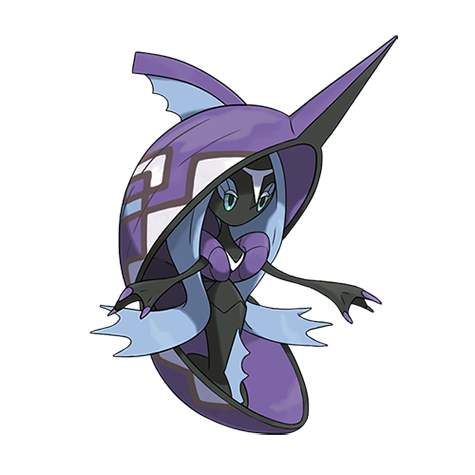
\includegraphics[width=\linewidth]{images/pokedex.png}
\end{minipage}
\begin{minipage}{0.45\linewidth}
Pokémon of the day:
\textbf{Tapu} (\#788) [Water].
This guardian deity of Poni Island manipulates water. Because it lives deep within a thick fog, it came to be both feared and revered.
\end{minipage}
\center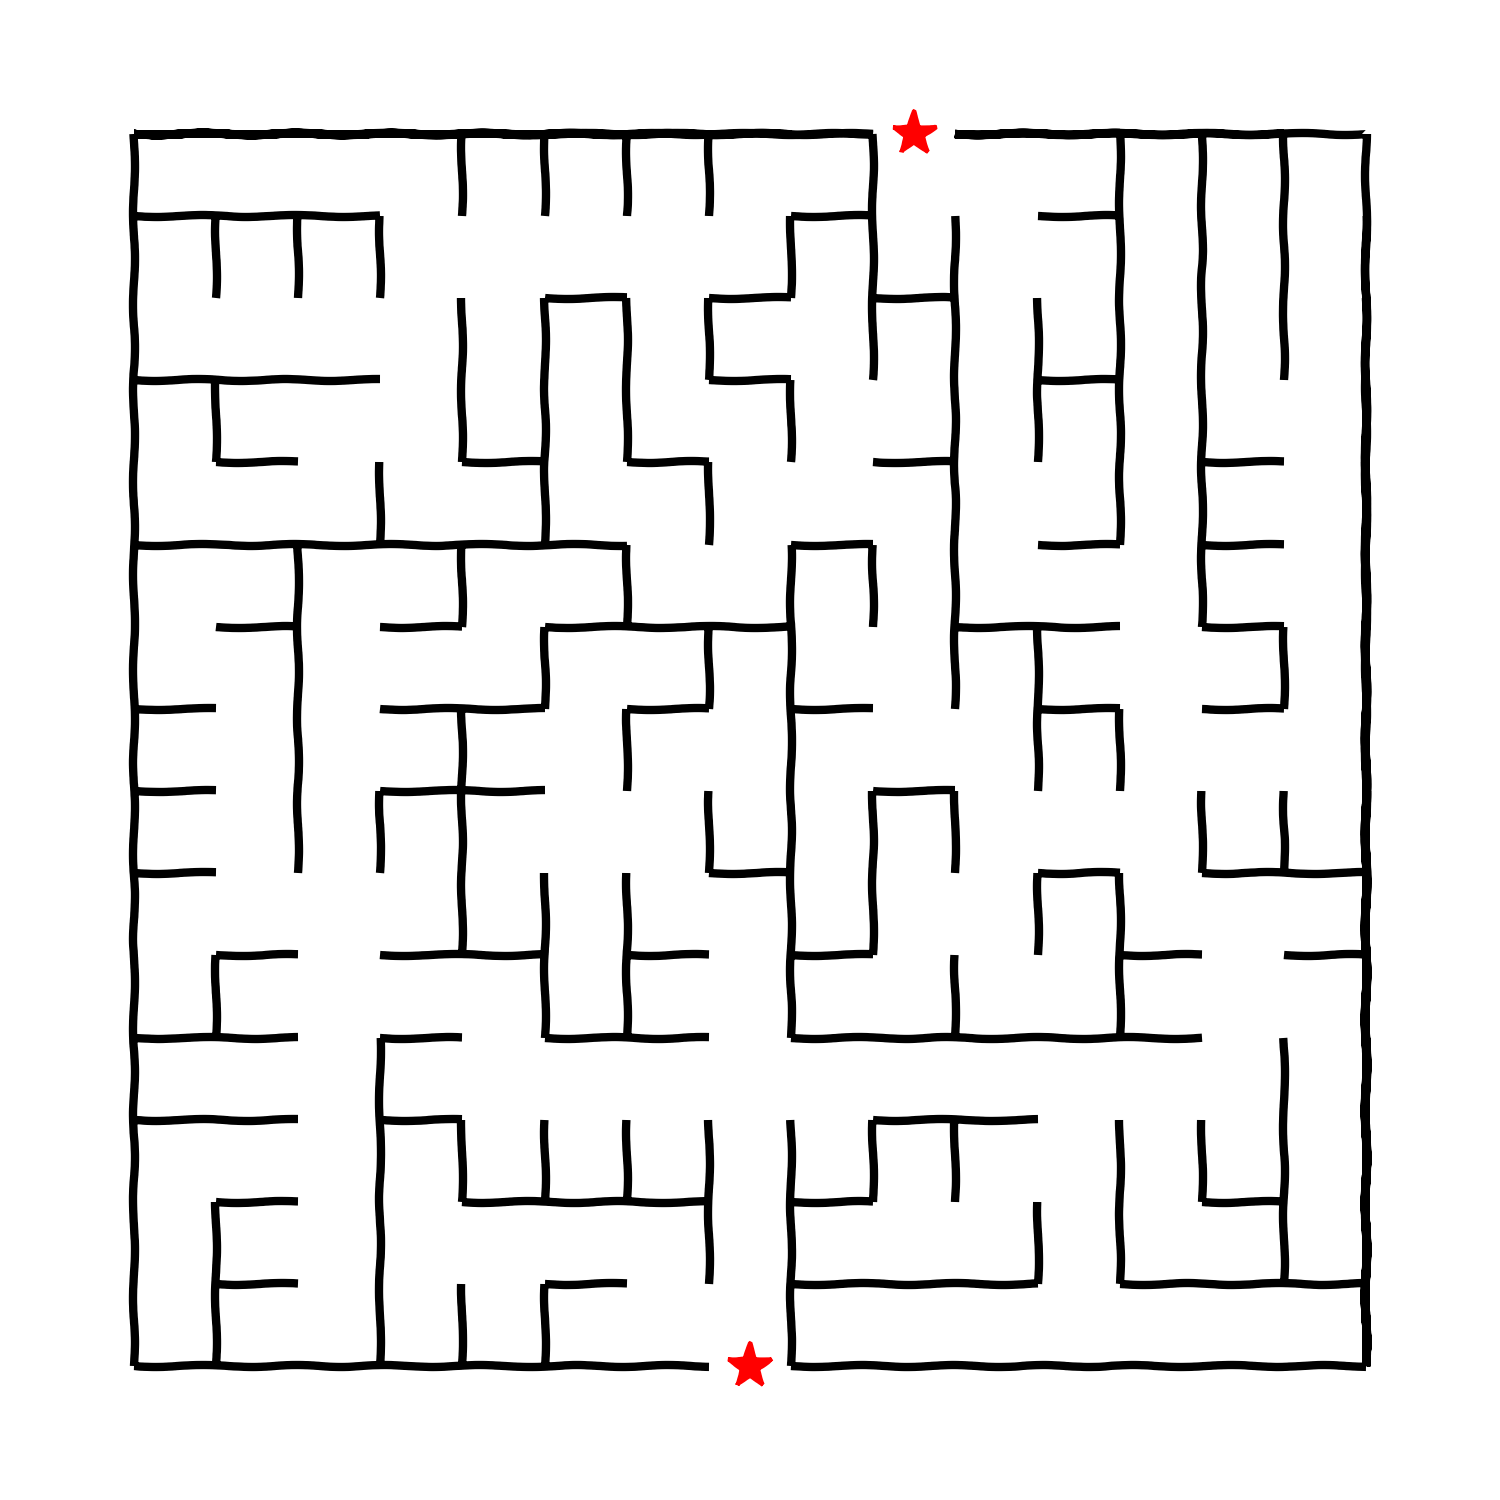
\includegraphics[width=\linewidth]{images/maze_j.png}

\renewcommand*\sudokuformat[1]{\sffamily#1}
\setlength\sudokusize{0.98\linewidth}
\setlength\sudokuthickline{1pt}
\begin{center}
	\begin{sudoku-block}| | | | | |2|9| | |.
| |4| |7| | |5| | |.
|8|7|9| | | | | | |.
| | | | |8| | |4| |.
|7| |8| |2| | | |6|.
| |1| | | | | |7| |.
|6| | |8| | |1|3| |.
| | | | | |3|4|6| |.
| |2|1|5|4| | | | |.
\end{sudoku-block}
\end{center}
\setlength\sudokuthickline{0.3pt}
\begin{center}
	\begin{sudoku-block}
| | | | |6| | | | |.
| | |1| | | | | | |.
| |1| | | | |2| | |.
| |2| | | | | | | |.
| |3|5| |5| |3| | |.
| | | | | | | | | |.
| | | | | |4| | | |.
| | | | | | | | | |.
| |4| | | | | | |6|.
\end{sudoku-block}
\end{center}
\center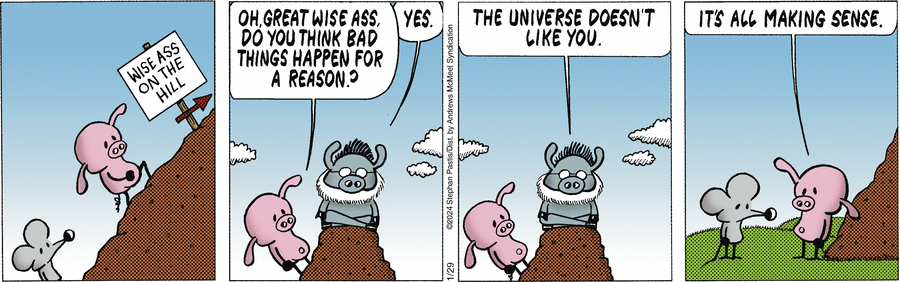
\includegraphics[width=\linewidth]{images/comic-pearls.png}
\center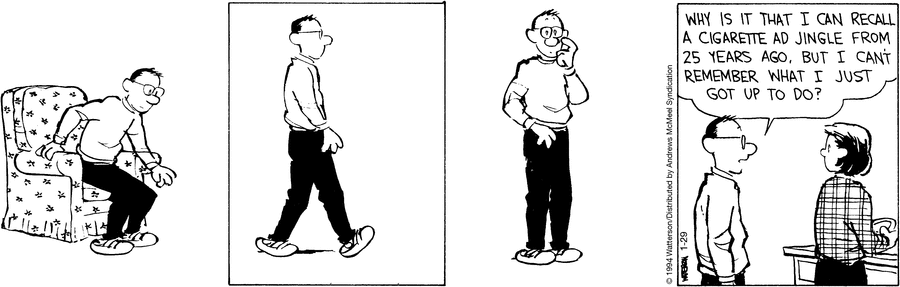
\includegraphics[width=\linewidth]{images/comic-calvinandhobbes.png}

\end{multicols}
\end{document}